%\documentclass[handout]{beamer}
\documentclass{beamer}

\usepackage[utf8]{inputenc}
\usepackage{default}

\usepackage{graphicx}
\usepackage{verbatim}
\usepackage{pgfpages}
\usepackage{epstopdf} % to have eps loaded
\usepackage[normalem]{ulem} % to have strike-through
\usepackage{alltt} % verbatim with commands inside
\usepackage{hyperref}

% \usepackage[latin1]{inputenc}
\usetheme{Warsaw}

% New commands
\newcommand{\cfgopt}[1]{{\it-*#1 config option}}
\newcommand{\signal}[1]{{\it#1}}
\newcommand{\feedback}[1]{{\tiny (#1 feedback)}}
\newcommand{\code}[1]{{\tiny #1)}}
\newcommand{\regbit}[1]{({\bf#1})}
\newcommand{\tclpackage}[1]{{\alert{#1}}}
%\newcommand{\octopus}{\includegraphics[height=2ex]{../logo/octobiwan.png}}

\title[Synthesis Flow]{Yet Another Synthesis Flow for RTL Compiler}
%\subtitle{Power Through Collaborative Design}

\author{Octavian Petre}
\institute{NXP Semiconductors}
\date{May 21, 2014}
\titlegraphic{\includegraphics[height=.15\textheight]{support_pictures/source/company_logo.jpg}}

\logo{\includegraphics[height=15px]{support_pictures/source/company_logo.jpg}}
% to have page numbers
% This is copied from /usr/share/texmf-site/tex/latex/beamer/base/themes/outer/beamerouterthemeinfolines.sty
% which is used in Madrid theme
\setbeamertemplate{footline}
{%
  \leavevmode%
  \hbox{%
  \begin{beamercolorbox}[wd=.333333\paperwidth,ht=2.25ex,dp=1ex,center]{author in head/foot}%
    \usebeamerfont{author in head/foot}\insertshortauthor(\insertshortinstitute)
  \end{beamercolorbox}%
  \begin{beamercolorbox}[wd=.333333\paperwidth,ht=2.25ex,dp=1ex,center]{title in head/foot}%
    \usebeamerfont{title in head/foot}\insertshorttitle
  \end{beamercolorbox}%
  \begin{beamercolorbox}[wd=.333333\paperwidth,ht=2.25ex,dp=1ex,right]{date in head/foot}%
    \usebeamerfont{date in head/foot}\insertshortdate{}\hspace*{2em}
    \insertframenumber{} / \inserttotalframenumber\hspace*{2ex} 
  \end{beamercolorbox}}%
  \vskip0pt%
}

\begin{document}
\setcounter{tocdepth}{1}


% to be added to presentation 
% 

\begin{frame}[plain]
\titlepage 
%\tiny{Get the latest presentation from \href{https://www.collabnet.nxp.com/integration/viewvc/viewvc.cgi/presentations/octopus.pdf?root=octopus&system=exsy1002&view=co}{\underline{Octopus Repository}}}\footnote{\tiny{login required}}                                           
\end{frame}

\AtBeginSection[]
{
	  \begin{frame}<beamer>
		    \frametitle{Outline}
		    \tableofcontents[currentsection,currentsubsection]
	  \end{frame}
}


\begin{frame}
	\frametitle{Outline}
	%\tableofcontents[pausesections]
	\tableofcontents
\end{frame}

% At a glance we want to understand everything
% A translator between the natural language and the TCL RC.
\section{Why Another RTL Compiler Synthesis Flow?}
\begin{frame}{Why Another RTL Compiler Synthesis Flow?}{Less Error Prone (1)}
	\begin{itemize}[<+->]
	\item \textbf{Increasing Complexity}: RC scripts tend to grow with new projects and methodologies. \\ \alert{I want to avoid long spaghetti code.}
	\item \textbf{Recommended Flow}: Cadence recommends certain steps in a certain order. \\ \alert{I want to check them easily.}
	\item \textbf{Missing Separation}: Customized steps/code are mangled with standard ones.\\ \alert{I want to focus on the customized ones.}
	\item \textbf{(Re)Set of Variables}: Variables (re)set in several places in different directory trees.\\ \alert{I want to avoid reading all scripts} 
	\end{itemize}
\end{frame}

\begin{frame}{Why Another RTL Compiler Synthesis Flow?}{Less Error Prone (2)}
	\begin{itemize}
	\item<1-> \textbf{Missing Collaboration}: Fixed issues are not always picked up by new designs. \\ \alert{I want to get all fixes fast.}
	\item<2-> \textbf{Insufficient Standardization}: 
		\begin{itemize}
		\item<2-> Flow steps.\\ \alert{I want clear flow steps}
		\item<3-> Few, no, or difficult to understand procedures. \\ \alert{I want clear API for procedures}.
		\end{itemize}
	\item<4-> More powerful procedures.
	\end{itemize}
\end{frame}


\section{Key Features - Summary}
\begin{frame}{Key Features - Summary}{1}
	\begin{itemize}[<+->]
	 \item \textbf{Highly Hierarchical}
		\begin{itemize}
		 \item Build on top of other custom developed TCL packages \href{https://github.com/octavsly/octopus}{GitHub/*/octopus}
		 \item Wraps and Extends standard RC commands (overloading allowed?). \\ Introduction of new procedures.
		\end{itemize}
	 \item \alert{Design Maturity Level}. Influences flow/attributes/reporting/etc. 
	 \item Follows the recommended Cadence RC synthesis flow.
	 \item Split of common from configurable TCL
		\begin{itemize}
		\item Goal is to minimize the configurable part without jeopardising the flexibility 
		\item \alert{Design configuration file} contains both \\ \alert{TCL variables} and \alert{TCL code}
		\end{itemize}
	\end{itemize}
\end{frame}

\begin{frame}{Key Features Summary}{2}
	\begin{itemize}[<+->]
	 \item \textbf{Automatic SDC Constraints Generation}. \\ DfT setup automatically translated from NXP specific information to SDC constraints.
	 \item \textbf{Automatic DfT setup from SDC constraints}. \\ Crawling RC database for set\_case\_analysis and clocks.
	 \item CPF based flow.
		\begin{itemize}
		\item libraries read via CPF
		\item constraints
		\item power intent
		\end{itemize}
	\item Custom colourful  messages tracing for alerting future flow users.
	\item Command line startup with user customizable options
	\item Source available at \href{https://github.com/octavsly/rtlcompiler}{GitHub/*/rtlcompiler}
	\end{itemize}
\end{frame}

\section{Key Features - Details}
\subsection{Highly Hierarchical}
\begin{frame}[fragile,plain]{Highly Hierarchical}{main.tcl (1)}
\begin{columns}
\begin{column}{0.5\textwidth}
\tiny
\begin{verbatim}	
include ./design_specific_input.tcl

# Setting RC attributes.
# Design maturity dependent
include rc_attributes.tcl

# Creating directories, cleaning files etc.
include house_keeping.tcl

#Library (including dont_use) and ple setup"
read_cpf -library $_CPF_FILE

include dont_use.tcl

include ple_setup.tcl

# Read, Elaborate and Check the Design"
include read_hdl.tcl

::octopusRC::elaborate

# Generate automatic constraints
include generate_constraints.tcl

#Read CPF in: 
#power information, modes and constraints
::octopusRC::read_cpf --cpf $_CPF_FILE

\end{verbatim}
\end{column}

\begin{column}{0.5\textwidth}
\tiny
\begin{verbatim}
#Define DFT and clock gating"
include dft_settings.tcl

include clock_gating_settings.tcl

#Synthesizing to generic
include design_constraints.tcl

# synthesize. Different levels are picked 
# based on design maturity level
::octopusRC::synthesize -to_generic

#Synthesizing to gates
::octopusRC::synthesize -to_mapped

#Connect scan chains
include connect_scan_chains.tcl

#Incremental Synthesis
include design_constraints_incremental.tcl

::octopusRC::delete_unloaded_undriven 

::octopusRC::synthesize -to_mapped -incremental
# Commit cpf
include ./commit_cpf.tcl
\end{verbatim}

\end{column}
\end{columns}
\end{frame}

\begin{frame}[fragile,plain]{Highly Hierarchical}{main.tcl (2)}
\tiny
\begin{verbatim}
#!/bin/sh
# the next line restarts using -*-Tcl-*-sh \
exec rc -64 -logfile rc.log -cmdfile rc.cmd -overwrite -f "$0" -execute "set argv \"\" ; set argv ${1+\"$@\"} ; set prog_name $0; set_attribute source_verbose true; set_attribute source_verbose_proc true ; set_attribute source_verbose_info true"

#This is the main RC script. It will source other files

if { [info exists env(OCTOPUS_INSTALL_PATH) ] } {
        lappend auto_path $env(OCTOPUS_INSTALL_PATH)
} else {
        puts "ERROR: Please set environmental variable OCTOPUS_INSTALL_PATH to point to the location of octopus.tcl file"
        exit 1
}


package require octopusRC 0.1
package require octopus   0.1

#::octopus::set_octopus_color --disable

set EXEC_PATH "" ; set DATA_PATH "" ; set CRT_LIB "" ; set CRT_CELL "" ; regexp {(.*/data/)([^/]+_lib)/([^/]+)/.*} [exec pwd] EXEC_PATH DATA_PATH CRT_LIB CRT_CELL
::octopus::add_option --name "--maturity-level" --valid-values "pre-alpha alpha beta release-candidate final" --help-text "Maturity level of the design."
::octopus::add_option --name "--design" --variable-name "DESIGN" --default "$CRT_CELL" --help-text "Top level design for which synthesis will be performed."
::octopus::add_option --name "--reports-path" --variable-name "_REPORTS_PATH" --default "[exec pwd]/rpt" --help-text "Directory holding the reports."
::octopus::add_option --name "--netlist-path" --variable-name "_NETLIST_PATH" --default "${DATA_PATH}/${CRT_LIB}/${CRT_CELL}/NETLIST" --help-text "Directory holding the netlist."
::octopus::add_option --name "--cpf" --variable-name "_CPF_FILE" --default "${DATA_PATH}/${CRT_LIB}/${CRT_CELL}/POWER/${CRT_CELL}.cpf" --help-text "CPF file location."
::octopus::add_option --name "--clean-rpt" --type "boolean" --default "false" --help-text "Clean all reports before the run. Otherwise reports are cleaned one by one."
::octopus::add_option --name "--run-speed" --default "slow" --valid-values "slow fast" --help-text "If set to fast a lot of reports will be skipped."

set ::octopus::prog_name $prog_name

::octopus::extract_check_options_data

::octopus::abort_on error --display-help
\end{verbatim}
\end{frame}

\subsection{TCL packages}
\begin{frame}{TCL packages}{In a nutshell}
\begin{columns}
\begin{column}{0.4\textwidth}
	\centering
	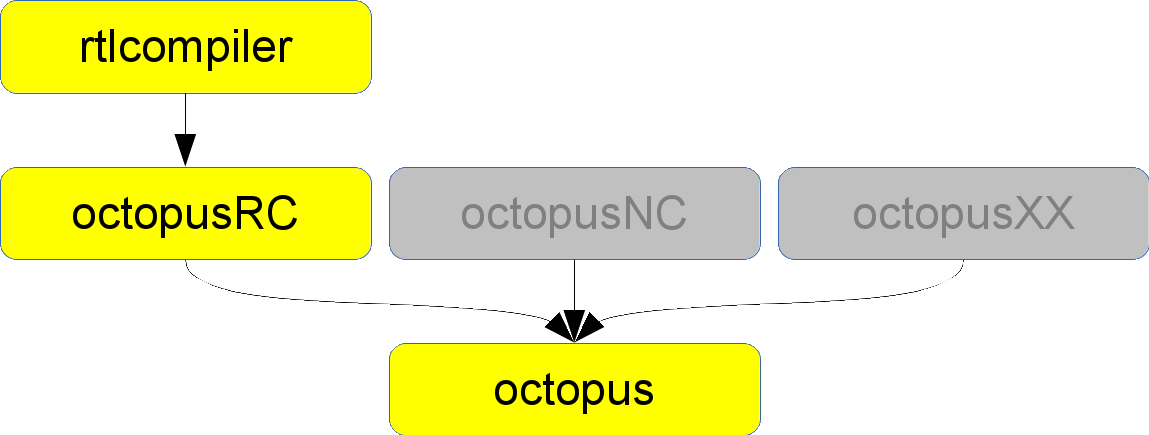
\includegraphics[width=\textwidth,height=0.6\textheight]{./support_pictures/export/TCL_packages.png}
\end{column}
\begin{column}{0.6\textwidth}
	\begin{itemize}
	 \item \textbf{rtlcompiler}
	 \item []<2-|alert@2>Synthesis scripts (e.g. {{main.tcl}}).
	 \item \textbf{octopusRC}
	 \item []<3-|alert@3>RTL Compiler TCL package. Depends on octopus package
	 \item \textbf{octopus}
	 \item []<4-|alert@4>TCL package: procedures to deals with argument parsing, error handling, colours, consistent look and feel throughout the flow, automatic help generation.
	\end{itemize} 
\end{column}
\end{columns}
\end{frame}

\subsection{OctopusRC package}
\begin{frame}{OctopusRC package}{Few Procedures (1)}
	\begin{itemize}
	\item \textbf{::octopusRC::delete\_unloaded\_undriven} 
	\item []<2-|alert@2>Deletes the unloaded and undriven. Depending on the design maturity this command is activated or not
	\item \textbf{::octopusRC::read\_dft\_abstract\_model}
	\item []<3-|alert@3>Reads CTL files and applies the information to all instances, avoiding name conflicts
	\item \textbf{::octopusRC::define\_dft\_test\_clocks} 
	\item []<4-|alert@4>Define DfT clocks from the clocks specified in a certain timing mode.
	\item \textbf{::octopusRC::define\_dft\_test\_signals}
	\item []<5-|alert@5>Define DfT signals from set\_case\_analysis.
	\end{itemize}
\end{frame}

\begin{frame}{OctopusRC package}{Few Procedures(2)}
	\begin{itemize}
	\item \textbf{::octopusRC::synthesize} 
	\item []<2-|alert@2> Additionally writes lec, db, reports, etc.
	\item \textbf{::octopusRC::set\_attribute\_recursive}
	\item []<3-|alert@3> Ideally should set attributes recursively to any type of object.\footnote{Not fully implemented}
	\item <4-> others ...
	\end{itemize}
\end{frame}

\subsection{Design Maturity Level}
\begin{frame}{Design Maturity Level}{1}
	\begin{itemize}[<+->]
	\item \textbf{::octopusRC::set\_design\_maturity\_level} \\pre-alpha, alpha, beta, release-candidate, final.
	\item RC attributes are differentiated as shown on slide~\ref{rc_attributes}.
	\item Synthesis optimization efforts are set at medium or high.
	\item Boundary optimization settings.
	\end{itemize}
\end{frame}


\begin{frame}[fragile,plain,label=rc_attributes]{Design Maturity Level}{2}
\begin{columns}
\begin{column}{1.1\textwidth}
\tiny
\begin{verbatim}
#TABLE HEADERS DESCRIPTION
#rc_attribute                           pre-alpha       alpha           beta    release-candidate       final           comment
show_report_options                     true            true            true            true            true            -
detailed_sdc_messages                   true            true            true            true            true            -
group_generate_portname_from_netname    true            true            true            true            true            -
lp_insert_clock_gating                  -               true            true            true            true            -
lp_insert_clock_gating_incremental      -               true            true            true            true            -
write_vlog_bit_blast_constants          true            true            true            true            true            -
information_level                       9               9               9               9               9               -
continue_on_error                       true            -               -               -               -               -
find_inefficient_use                    true            true            true            -               -               -
log_command_error                       true            true            true            -               -               -
report_tcl_command_error                true            true            true            -               -               -
source_verbose                          true            true            -               -               -               -
source_verbose_proc                     true            true            -               -               -               -
source_verbose_info                     -               false           -               -               -               -
source_suspend_on_error                 -               true            true            -               -               -
hdl_report_case_info                    true            true            true            -               -               -
hdl_track_filename_row_col              true            true            true            -               -               -
hdl_array_naming_style                  %s_%d_          %s_%d_          %s_%d_          %s_%d_          %s_%d_          %s_%d_
hdl_instance_array_naming_style         %s_%d_          %s_%d_          %s_%d_          %s_%d_          %s_%d_          %s_%d_
hdl_record_naming_style                 %s_%s_          %s_%s_          %s_%s_          %s_%s_          %s_%s_          %s_%s_
hdl_generate_index_style                %s_%d_          %s_%d_          %s_%d_          %s_%d_          %s_%d_          %s_%d_
hdl_generate_separator                  __              __              __              __              __              __
#write_vlog_empty_module_for_black_box  true            true            -               -               -               -
delete_unloaded_insts                   false           false           -               -               -               -
delete_unloaded_seqs                    false           false           -               -               -               -
...
\end{verbatim}
\end{column}
\end{columns}
\end{frame}

\begin{frame}[fragile,plain]{Design Maturity Level}{2}
\begin{columns}
\begin{column}{1.1\textwidth}
\tiny
\begin{verbatim}
#TABLE HEADERS DESCRIPTION
#rc_attribute                           pre-alpha       alpha           beta    release-candidate       final           comment
...
hdl_preserve_unused_registers           true            true            -               -               -               -
hdl_track_module_elab_memory_and_runtime true           -               true            true            -               -
dp_postmap_downsize                     -               -               true            true            true            -
dp_postmap_upsize                       -               -               true            true            true            -
fail_on_error_mesg                      -               -               -               true            true            -
boundary_optimize_invert_hier_pins      -               -               -               true            true            -
boundary_optimize_constant_hier_pins    false           -               -               -               -               -
dp_rewriting                            -               -               -               advanced        advanced        "LEC might fail. In that case use basic"
hdl_error_on_blackbox                   -               -               -               true            true            -
hdl_error_on_logic_abstract             -               -               -               true            true            -
hdl_unconnected_input_port_value        -               -               0               0               0               "do we need none(default) for all cases?"
hdl_undriven_output_port_value          -               -               0               0               0               "do we need none(default) for all cases?"
hdl_undriven_signal_value               -               -               0               0               0               "do we need none(default) for all cases?"
iopt_enable_floating_output_check       true            true            true            true            true            -
iopt_ultra_optimization                 -               -               -               true            true            -
glo_redrem_ultra_effort                 -               -               true            true            true            "hidden switch which explodes the runtime but removes most of the redundancy in the design."
optimize_constant_0_flops               false           false           -               -               -               -
optimize_constant_1_flops               false           false           -               -               -               -
optimize_constant_latches               false           false           -               -               -               -
optimize_merge_flops                    false           false           -               -               -               -
optimize_merge_latches                  false           false           -               -               -               -
propagate_constant_from_timing_model    false           false           -               -               -               -
tns_opto                                -               -               true            true            true            -
ultra_global_mapping                    -               -               true            true            true            -
dft_identify_internal_test_clocks       no_cgic_hier    no_cgic_hier    -               -               -               -
dft_report_empty_test_clocks            true            true            true            true            true            -
dft_shift_register_identification_mode  logical_only    logical_only    logical_only    logical_only    logical_only    "Other options are a bit more dangerous"
\end{verbatim}
\end{column}
\end{columns}
\end{frame}

\subsection{Configuration File}
\begin{frame}{Split Common from Configurable TCL Code}{1}
	\begin{itemize}[<+->]
	 \item Group the configurable part in one file
	 \item Allow both TCL variables and TCL code \\ Reading HDL files, LEF's, reading CTL's, scan-enable specification, scan-chains setup, constraints generation, test-point insertion
	\end{itemize}
\end{frame}

\begin{frame}[fragile,plain]{Configuration File}{1}
\begin{columns}
\begin{column}{1.1\textwidth}
\tiny
\begin{verbatim}
namespace eval diehardus {
# File containing the RTL files. Supported formats rc,text,utel
variable read_hdl                "::octopusRC::read_hdl --type rc ../rtlcompiler/cmd/read_hdl.tcl"

variable lefs "
                 $env(CADENV_HOME)/.caddata/krfdi/tools/cadence_edi/xkrfdix_5.6.lef\
...

variable read_ctl {
                  ::octopusRC::read_dft_abstract_model\
                          -assume_connected_shift_enable\
                          --ctl \
                                  $env(PROJECT_WORK)/data/hrxc_hrxc1_lib/hrxc_hrxc1/catviews/hrxc_hrxc1_ana_tpr.ctl \
                                  $env(PROJECT_WORK)/data/hrxc_hrxc2_lib/hrxc_hrxc2/catviews/hrxc_hrxc2_ana_tpr.ctl \
                                  $env(PROJECT_WORK)/data/hrxc_hrxc2_lib/hrxc_hrxc2/catviews/hrxc_hrxc2_trim_tpr.ctl \
                                  ... \
                          --boundary-opto \
                          --debug-level 2

                  ::octopusRC::read_dft_abstract_model \
                          --ctl \
                                  $env(PROJECT_WORK)/data/ltthf_lib/ltthf_asdopefsd_asdcsda/TEST/ltthf_asdopefsd_asdcsda_chains.ctl \
                          --debug-level 2
                  }
...
}
\end{verbatim}
\end{column}
\end{columns}
\end{frame}

\begin{frame}[fragile,plain]{Configuration File}{2}
\begin{columns}
\begin{column}{1.1\textwidth}
\tiny
\begin{verbatim}
...
set scan_chains_insertion {
                # Define floating segment with falling edge FF's. They will be put in front of the chain.
                define_dft floating_segment \
                        -name falling_edge_flops [::octopus::find_fall_edge_objects]

                ## Define scan chains
                define_dft scan_chain \
                        -name allFF_0 \
                        -sdi I0/u0_hrxc_ic_core_test/si[0] \
                        -sdo I0/u0_hrxc_ic_core_test/so[0] \
                        -non_shared_output \
                        -head falling_edge_flops \
                        -terminal_lockup level_sensitive

                define_dft scan_chain \
                        -name allFF_1 \
                        -sdi I0/u0_hrxc_ic_core_test/si[1] \
                        -sdo I0/u0_hrxc_ic_core_test/so[1] \
                        -non_shared_output \
                        -terminal_lockup level_sensitive

                connect_scan_chains -incremental

                fix_scan_path_inversions allFF_0
                fix_scan_path_inversions allFF_1
}
...
\end{verbatim}
\end{column}
\end{columns}
\end{frame}

\subsection{Automatic SDC Constraints Generation}
\begin{frame}{Automatic SDC Constraints Generation}
	\begin{itemize}[<+->]
	 \item NXP DfT: Use of serial shift registers, containing test-data file describing the static values during test.
	 \item By parsing these test data files, already a big chunk of constraints can be automatically generated.
	 \item Generated constraints used at least in three timing modes \textbf{scan-shift}, \textbf{capture} and \textbf{functional}.
	\end{itemize}
\end{frame}

\subsection{Automatic DfT Setup from SDC Constraints}
\begin{frame}{Automatic DfT Setup from SDC Constraints}
	\begin{itemize}
	 \item<1-> \textbf{Clocks} {{::octopusRC::define\_dft\_test\_clocks}}
		\begin{itemize}
		\item<2-|alert@2> Specify the timing mode
		\item<3-|alert@3> Clocks are extracted from RC database 
		\item<4-|alert@4> Clocks can be added or removed (not recommended).
		\end{itemize}
	\item<1-> \textbf{Test Signals} {{::octopusRC::define\_dft\_test\_signals}}
		\begin{itemize}[<+->]
		\item<2-|alert@2> Specify the timing mode
		\item<3-|alert@3> Extract the set\_case\_analysis from RC database
		\item<4-|alert@4> Signals to add or remove (not recommended)
		\end{itemize}
	\end{itemize}
\end{frame}

\section{Conclusion}
\begin{frame}{Conclusion}{Things to Remember}
	\begin{itemize}[<+->]
	\item RTL Compiler Synthesis flow
	\item Highly hierarchical (scripts and two other TCL packages)
	\item Customization part of the flow is in a single file and contains both variables and code
	\item Generate DfT related SDC from NXP specific test-data files
	\item Generate DfT constraints from SDC.
	\item CPF only flow
	\item \alert{Flow and packages freely available at \href{https://github.com/octavsly/}{GitHub} \\ Can be extended as needed (e.g. technology exploration)}
	\end{itemize}
\end{frame}

\begin{frame}
\alert{\centerline{{\huge Questions?}}}
\end{frame}
\end{document}
           
